\documentclass{report}
\usepackage[utf8]{inputenc}
\usepackage{cite}
\usepackage[english]{babel}
 \usepackage{xcolor}
\usepackage{minted}
\usepackage{graphicx}
\usepackage{dirtytalk}
\usepackage{float}
\usepackage{appendix}
\usepackage{tikz}
\usepackage{caption}
\usepackage{gensymb}
\usepackage{lmodern}
\usepackage{multirow}
\usepackage{booktabs}
\usepackage{array}
\usepackage{adjustbox}
\usepackage{upquote}
\usepackage{amsmath}
\usepackage{titlesec}
\usepackage[hidelinks]{hyperref}
\usepackage{fancyhdr}
\usetikzlibrary{mindmap,shadows, shapes, arrows, positioning}




%% Change these:
\newcommand{\projecttitle}{ An Exploration of Shared Augmented Reality and its Application in Architecture }
\newcommand{\projectauthor}{Daire Ní Chatháin}
\newcommand{\projectadvisor}{Dr. Brian McGinley}
\newcommand{\projectprogramme}{B.Sc.(Hons) in Software Development}
\newcommand{\projectdate}{\today}
%% End of things to change.



\tikzstyle{rect} = [rectangle, fill=blue!50, text width=4.5em, text centered, minimum height=4em, rounded corners]
\tikzstyle{line} = [draw, ->, very thick]
\tikzstyle{oval} = [ellipse, fill=green!50, text width=5em, text centered]

\newcolumntype{x}[1]{>{\centering\arraybackslash\hspace{0pt}}p{#1}}


\begin{document}
  \begin{titlepage}
    \begin{minipage}[t][4cm]{\textwidth}
      \centering
      \rule{\linewidth}{0.5mm} \\[0.4cm]
      { \LARGE \bfseries \projecttitle \\[0.4cm] }
      \rule{\linewidth}{0.5mm} \\[0.8cm]
    \end{minipage}
    
    \begin{minipage}[t][6.5cm]{\textwidth}
      \centering
      \textbf{\projectauthor}\\[0.4cm]
      \projectprogramme
    \end{minipage}
  
    \begin{minipage}[t][1cm]{\textwidth}
      \centering
      \textsc{\projectdate}
    \end{minipage}
      
    \begin{minipage}[t][3cm]{\textwidth}
      \centering
      \textbf{Final Year Project}\\[0.3cm]
      Advised by: \projectadvisor \\[0.1cm]
      Department of Computer Science and Applied Physics\\
      Galway-Mayo Institute of Technology (GMIT)
    \end{minipage}

    \begin{center}    
      
\includegraphics[scale=0.7]{./images/gmit.png}
    \end{center}
  \end{titlepage}
  \setcounter{page}{1}
\
\tableofcontents
\begin{abstract}

Shared augmented reality, is an emerging technology showing promising value in a wide range of disciplines. This project seeks to examine shared augmented reality through the lens of its value in the field of architecture. 
In the first section of this dissertation, an investigation into the current tools available for the creation of shared augmented reality experiences is conducted. An evaluation of these tools is completed highlighting how each tool can be applied to implement a multi-user augmented reality experience. Following this, a selection of technologies are applied to create a cross-platform mobile application featuring shared augmented reality functionality, for use in architecture. To conclude, the shared-augmented reality system is presented and evaluated. 
   
\end{abstract}

 \chapter{Introduction}
 AR(AR) is an emerging trend in the field of computing. AR’s growing popularity can partially be attributed to the rise of mobile phone use and a shift in AR applications no longer requiring expensive hardware and sophisticated equipment, such as head-mounted displays. Shared AR is a relatively new concept. It extends AR technologies, connecting multiple users together in order to create a synchronized, augmented space. This introduces a social, collaborative aspect to AR that lends itself to a range of use cases, from multiplayer gaming to training and education. Given the variety of exciting use cases for collaborative AR experiences, there has been significant advancements in the area. Tech giants such as Google and Apple are investing heavily in the sector, recently releasing software development kits for the creation of such AR experiences \cite{arcore} \cite{arkit}. In an attempt to evaluate the state of the field, the primary goal of this project is to investigate the various approaches and technologies currently used to implement multi-user AR experiences.

The field of architecture was selected as an ideal use case for demonstrating the value shared AR can provide. The architecture sector is an area requiring 3D visualizations and a need for common understanding and communication between client and architect. This project aims to highlight how these requirements can aptly be fulfilled through the use of shared AR, delivered via a cross-platform mobile application. An example use case could be an architect wishing to discuss architectural plans with a client. Each of the involved parties open up the mobile application and view the proposed architectural model in a shared augmented space. The model can be modified, re-positioned and scaled and the resulting changes will be viewed by all parties in the same shared AR space.  


\section{Context}
\subsection{AR}
Augmented (AR) is a 3D technology that enhances the user’s sensory perception of the real world with a contextual layer of information  \cite{azuma1997survey}. According to \cite{martin2015augmented}, the key to creating successful AR experiences lies in the smooth combination of the actual and virtual world. This merging of the real and virtual can be achieved using a variety of tools and methodologies. 

The primary method of implementing AR experiences is through the use of mobile devices and AR software development kits. Mobile devices offer an ideal hardware platform for AR applications. The portability, encouragement of high social interactivity, and independent operability \cite{hwang2012context} make mobile devices an attractive platform for AR applications. For this reason, it was decided that implementing shared AR in this project should be done via a mobile application. 

\subsection{Shared AR}
Shared AR or multi-user AR, allows multiple users to share a synchronized augmented space. Users see the same digital content simultaneously, creating a shared social experience that engages the users with the content, and with each other.  Each user can view the digital content from their own perspective – a user on one side of the room may see the front, while a user on the other side sees the rear. 


\section{Project Objectives}
The primary goal of this project is to demonstrate shared AR through the medium of a mobile application. The mobile application is intended to be used by architects and their clients as a means of promoting communication and collaboration between these parties.

\begin{itemize}
    \item Evaluate and establish the current tools available for creating cross-platform multi-user AR mobile applications.
    \item Implement shared AR.
    \item Build a full stack system for use in architecture, featuring shared AR technologies. 
\end{itemize}

\section{Summary} 
In this section a brief description of each chapter in this dissertation is provided. 

\subsection{Background}
This chapter describes the various technologies used during the development of this project. These technologies range from project management to database tools, to mobile application development frameworks. An evaluation of AR software development tool kits is also conducted in this chapter

\subsection{Methodology}
This chapter outlines the processes undertaken during the various stages of the project’s planning and development. It also describes the manner in which decisions regarding design and implementation were conducted. 

\subsection{System Design}
In this chapter, a detailed explanation of the overall system architecture is provided. The system’s key components are discussed and broken down into their underlying technologies. 

\subsection{System Evaluation}
This chapter evaluates the implemented system in terms of the initial project objectives. Final results are reviewed, along with a discussion on opportunities for improvement within the overall system.  

\subsection{Conclusion}
To conclude, a brief overview of the implemented system is provided. Key insights gained during the project's development are reflected upon and discussed.

%%%%%%%%%%%%%%%%
% Chapter 1
%%%%%%%%%%%%%%%%
\chapter{Background}

\section{Project Management}
\subsection{Agile}
First described in the Manifesto for Agile Software Development \cite{beck2001manifesto}, Agile development is a set of principles and methods for project management. The Agile methodology is characterized by an iterative, approach to software development \cite{cockburn2001agile}. There is a strong emphasis on embracing the change and uncertainty normally associated with software development projects. The goal is to continuously deliver working software while simultaneously refactoring and tweaking as the development process unfolds.  

\subsubsection{Kanban}
The Kanban method is highly visual and aims to illustrate each stage within a process and the interconnectedness between them \cite{sugimori1977toyota}. The basic structure of the Kanban system is a storyboard. The board is split into different lists that represent the consecutive stages of completing the work. Within each list are cards. These are the smallest work units, or simply put, a task. The Kanban process, in essence, is moving a card (a single task) from left to right on the board. On the left-most side is the To Do list – and the task is gradually pushed to completion until it reaches the Done list. Because the board offers a clear overview of all tasks and their progress, it’s easy to see where any work gets stalled

\subsubsection{SCRUM}
The SCRUM method is based on the work of Pittman and Booch \cite{pittman1993lessons}. The focus of Scrum is addressing software development in a flexible way through the use of \say{inspect and adapt feedback loops}. Time is divided into short work cadences, known as sprints, typically one week or two weeks long.  At the end of each sprint, stakeholders and team members meet to discuss the progress of the previous sprint and plan for the next sprint. 


\section{Tech Review}

The following section outlines the key tools and technologies used during the development of this project.


\subsection{Project Management Tools}

\subsubsection{Github}
Git is an open source distributed version control system that allows content to be tracked by maintaining a history of changes. GitHub is a code hosting platform that implements Git for version control and collaboration.
\subsubsection{Trello}
Trello is an online project management tool that facilitates the creation of storyboards. A storyboard can represent a stream of activity or an entire project. Boards, lists and tasks can be created via Trello's user interface. 


\subsection{Developer Tools}

\subsubsection{Atom Editor}
Atom is a free, open source text editor. It features support for Windows, Linux and macOS, and takes the form of a desktop application. Built using Electron, CoffeeScript and HTML, Atom’s key feature is its customizability. Developers are encouraged to write their own plugins and as a result, it has been dubbed the \say{Hackable editor of the 21st century}\cite{atom}.
Github is the chief contributor to the Atom project and as a result, Atom has Github integrated at its core. The GitHub package for Atom allows developers to create new branches, stage and commit, push and pull, resolve merge conflicts, view pull request - all from within the editor. 


\subsubsection{Nuclide}
Nuclide is a set of packages that adds IDE-like functionality to Atom. Developed by Facebook, Nuclide is built on top of Atom’s source code, providing pre-configured optimizations and customizations. Nuclide has strong support for web and mobile development. While Nuclide has been shown to consume more memory than Atom alone, it adds substantial functionality.\cite{nuclide} 

\subsubsection{Quick Open}
Quick Open is one of the most notable features of Nuclide. The Quick Open technology gives access to Nuclide’s file search mechanism, including OmniSearch, which quickly displays recently opened files, quick searches for files based on partial names, and depending on the project, can search within files for symbols\cite{quickopen}.


\subsubsection{Unity}
Unity is a cross-platform real-time engine developed by Unity Technologies. Unity allows developers to create games and interactive experiences in both 2D and 3D. The central scripting API is compatible with the C\# programming language. The Unity editor supports the creation of content for a wide variety of platforms ranging from gaming consoles to mobile devices on Android, iOS, and Windows \cite{unity}. 

\subsubsection{Android Studio}
Android Studio is the de-facto IDE for developing Android applications. Android Studio features gradle-based build support, refactoring tools, lint tools, a virtual android device emulator and built-in support for the Google Cloud Platform and Firebase. It also supports development in all languages of IntelliJ, for example, Java, Koltin and C++. Android studio is supported on Microsoft Windows, Mac Os and Linux distributions \cite{android_studio}. 


\subsection{Application Development Tools}

\subsubsection{Typescript}
TypeScript is a superset of JavaScript which provides functionality for static typing, classes and interfaces \cite{typescript}. The core purpose of Typescript is to enable IDEs to provide developers with a more complete development environment.  The IDE is informed in real-time by the TypeScript compiler on its rich type information. This allows the developer to catch bugs and errors early in development. Furthermore,  static typing helps establish a more robust codebase.

\subsubsection{Typescript Compiler}
 Typscript code is transcompiled into regular JavaScript and can then be executed in any JavaScript engine (e.g. a browser). As TypeScript is a superset of JavaScript, existing JavaScript programs are also valid TypeScript programs. 

\subsubsection{Node}
NPM(Node Package Manager) is a software package manager and installer. It is the world’s largest software registry and contains over 800,000 code packages \cite{npm}. While NPM is primarily used to share open source software, many organizations use it to manage private development. NPM packages are defined in JSON and stored in a  package.json file. The management of dependencies can also be handled by npm. Dependencies are defined and shared in the package.json file. 

To install NPM, Node.js must be present on the machine. Node.js is a free, open-source server environment. It supports a myriad of platforms including Windows, Linux, Unix, Mac OSX and more.  The name npm (Node Package Manager) stems from when npm first was created as a package manager for Node.js.


\subsubsection{Angular JS}
Angular JS is an open source JavaScript framework used for front-end development. Its goal is to help manage the complexity associated with client-side javascript code. Angular JS extends the traditional functionality of HTML through the use of additional attributes to make the code more responsive and expressive \cite{angularjs}. 
 AngularJS teaches the browser new syntax through a construct called directives. Data binding and dependency injection are examples of such constructs. They function to eliminate much of the code otherwise needed to write dynamic applications.


\subsubsection{Apache Cordova}
Apache Cordova is a mobile application development framework. It is free, open sourced and supports the development of applications using CSS, HTML and Javascript. Leveraging these web technologies, Cordova creates hybrid applications that can run on a variety of platforms, including Android, iOS and Windows \cite{cordova_docs}. 

\begin{figure}[!ht]
\caption{Apache Cordova Architecture \cite{cordova_docs}}
\centering
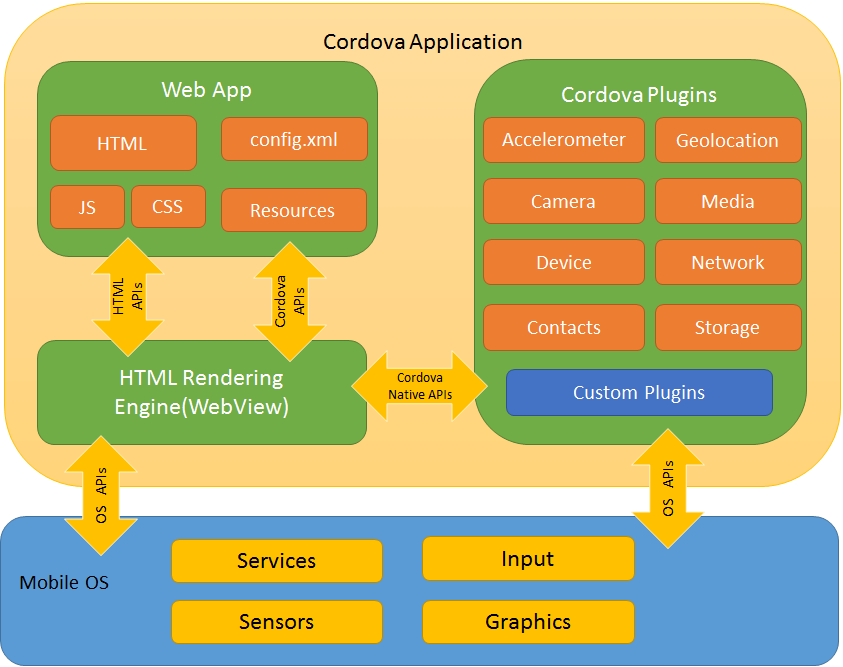
\includegraphics[width=1\textwidth]{images/apache_cordova.png}
\end{figure}

Apache Cordova applications execute within wrappers targeted to each platform.  HTML5 code is embedded inside a native WebView on the device, this interface is then used to access the device’s native resources. CSS3 and HTML5 are used for rendering the application content, while JavaScript is used to develop the application logic. HTML5 provides access to underlying hardware such as the accelerometer, camera, and GPS via the use of plugins. Plugins allow developers to add native functionality via the use of Javascript to communicate directly between the native layer and the HTML5 page. 


\subsubsection{Ionic Framework}
Ionic is a free, open-source mobile SDK for developing both native and web applications. Ionic builds on top of Apache Cordova, providing tools and services for developing hybrid applications through the use of web technologies \cite{ionidocs}. The framework is built on top of AngualJs and Apache Cordova. However, recent releases allow the developer to chose from React(Javascript Library), Angular(web framework) or Vue.js(Javascript library) as a user interface framework. Ionic utilises Cordova plugins to gain access to native hardware features such as camera, GPS, accelerometer. Ionic provides a set of front-end components and services while Cordova plugins access to native hardware of the device. Combined, Ionic and Cordova create  ‘native feeling’ applications. 

\subsubsection{Ionic CLI}
The Ionic CLI tool quickly scaffolds Ionic apps and provides a number of helpful commands to developers \cite{ionicli}. Ionic can be installed and updated via the CLI. Additionally, the CLI comes with a built-in build and debugging tools and a development server. Most of the tooling in the CLI is based on Node and is managed through npm.

\subsection{3D Modeling Tools}

\subsubsection{Blender}
Blender is a  suite of tools that support the creation of animated films, visual effects, art, 3D printed models, interactive 3D applications and video games \cite{blender}. Blender’s functionality includes 3D modelling, UV unwrapping, texturing, raster graphics editing, rigging and skinning, fluid and smoke simulation, particle simulation, soft body simulation, sculpting, animating, match moving, rendering, motion graphics, video editing and compositing. Blender’s software is open source and supported on Windows, MacOs and Linux distributions. 

\subsubsection{Wikitude Encoder}
3D content within Wikitude is managed and created using Wikitude 3D format files(.wt3). This is a compressed binary format for describing 3D models, optimized for fast loading and handling of 3D content on mobile devices. The Wikitude encoder converts 3D models into a flattened representation that can be rendered and augmented using the Wikitude SDK. The converter supports mesh-based 3D models so  that animations, textures and light sources can be applied \cite{wikiencoder}. 


The Wikitude encoder is a desktop application, supported on Windows, MacOs and Linux distributions. It currently only supports the input of .FBX for WT3 conversion. However, most 3D modelling tools support exporting to .FBX format, so files can readily be prepared for encoding. 
\begin{figure}[!ht]
\caption{Wikitude Encoder Desktop Application}
\centering
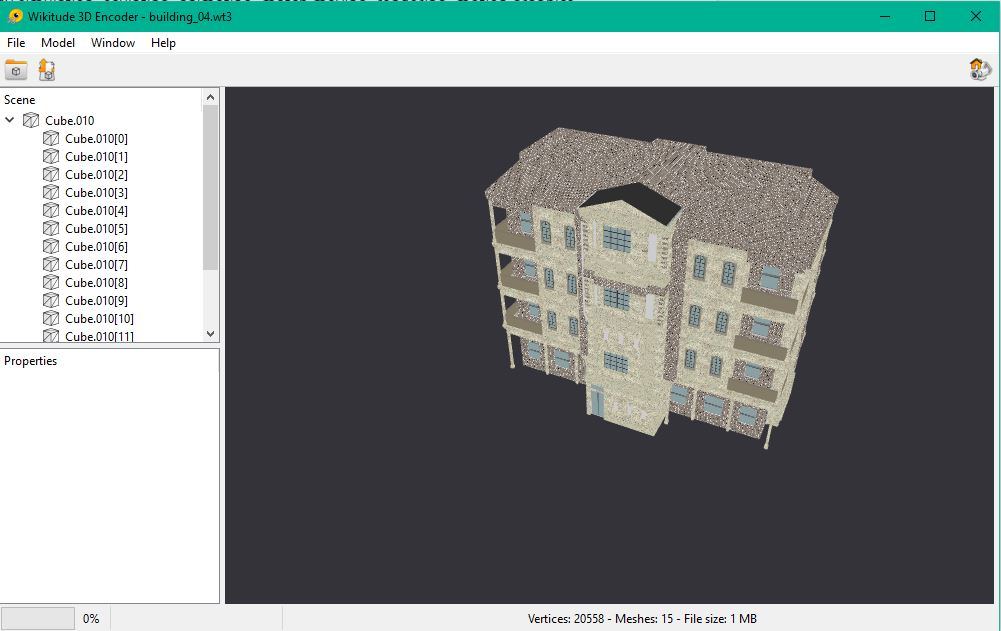
\includegraphics[width=1\textwidth]{images/wikitude_encoder.JPG}
\end{figure}


\subsection{Testing Tools}
\subsubsection{Selenium}
Selenium is a testing framework developed for web applications. Selenium is open sourced and supported on Windows, MacOs and Linux distributions. The selenium IDE is an integrated development environment (IDE) designed for creating and executing Selenium tests. It is implemented as a Firefox Add-On and as a Chrome Extension. It and allows for recording, editing, and debugging of functional tests\cite{selenium}.

\subsection{Database}

\subsubsection{Firebase}
Firebase is a platform developed by Google that provides developers with a range of tools and services to enhance mobile and web applications. Some of the features provided by Firebase include Real-time Databases, Authentication, Analytics, Hosting and Advertising\cite{firebase}. 
 \subsubsection{ Real-time Database}
The Firebase Realtime Database is a cloud-hosted NoSQL database that allows data to be stored and synced between users in real time\cite{firebase_realtime}. The database is in essence, a single JSON object. All clients share this one Real-time Database instance and automatically receive updates with the newest data.

 \subsubsection{Cloud Firestore}
Cloud Firestore is a scalable database from Firebase and  the Google Cloud Platform. Like the Firebase Realtime Database, it keeps data in sync across client apps through realtime listeners . It differs from the  real-time database in that you can upload documents and larger files for storage.

\subsection{Augmented Reality SDKs}
A selection of the top Augmented Reality SDKs were reviewed and evaluated in terms of their performance and features. The following research questions were used as criteria to examine their suitability for this project:

\begin{enumerate}
  \item What are the processes involved to implement basic AR?
\item How does it implement shared AR?

\end{enumerate}

\subsection{ARCore}

ARCore is a platform created by Google to facilitate the creation of augmented reality experiences. Using various API’s, ARCore enables mobile devices to generate a map of its environment which can then be manipulated with superimposed digital content.

ARCore makes use of the camera and sensors of the mobile device to integrate virtual content with real world surroundings. This merging of the real and virtual is achieved through three key techniques - motion tracking, environmental understanding and light estimation.



\subsubsection{Motion tracking}
 ARCore uses a process called concurrent odometry and mapping, or COM, to understand where the phone is relative to the world around it. ARCore detects visually distinct features in the captured camera image called feature points and uses these points to compute its change in location. The visual information is combined with inertial measurements from the device's IMU to estimate the pose (position and orientation) of the camera relative to the world over time. By aligning the pose of the virtual camera that renders your 3D content with the pose of the device's camera provided by ARCore, developers are able to render virtual content from the correct perspective.
 
 \subsubsection{Environmental understanding}
 ARCore creates an understanding of its environment using feature points. ARCore identifies clusters of feature points in areas containing vertical surfaces and horizontal lying objects, such as walls or tables. These surfaces are then converted into planes. ARCore identifies the boundaries of these planes, making them available to the application. This data can then be used to create an environment where virtual objects can be arranged, imparting the impression that the virtual objects are resting on the flat, real-world surface.

Using feature points to detect planes proves successful in most scenarios, however surfaces without discernible texture, for example - a white wall, may not be detected properly.

\subsubsection{Light estimation}
To create a sense of realism in the augmented reality scene, ARCore employs light estimation. Light estimation utilises the phone’s ambient light sensor in conjunction with the camera to estimate the current environment’s lighting conditions. This information is then made available to the application where colour correction and light intensity can be used to adjust the virtual objects such that they are under the same conditions as the environment.

 \subsubsection{ARCore Scenform Plugin}
 Sceneform is an Android Studio plugin for importing, viewing and building 3D assets\cite{sceneform}. Sceneform makes it straightforward to render realistic 3D scenes in AR and non-AR apps, without having to learn OpenGL. It features a high-level scene graph API and a realistic physically based renderer provided by Filament. 

\subsection{Sample Application with Sceneform \& ARCore}
For the purpose of this project, a period of time was spent investigating and developing applications using ARCore. This time was used to explore the viability of ARCore as the primary augmented reality SDK for this project.

\subsubsection{Permissions}
ARCore requires the use of the mobile device’s camera to superimpose its AR content. For this reason, the AndroidManifest.xml must be modified to indicate the application needs camera permission. 

\begin{minted}
[
baselinestretch=1.2,
fontsize=\footnotesize,
linenos
]
{xml}
<uses-permission android:name="android.permission.CAMERA" />
\end{minted}

\subsubsection{Renderables}
Sceneform uses Renderables to manage 3D content during the creation of an Augmented Reality scene. Renderables are 3D models that can be placed in any location within the scene. They consist of materials, textures and meshes. In this sample app, a renderable was created using a .obj asset file and an associated sceneform asset file.


\subsubsection{Sceneform Assets}
The Sceneform Asset Definition (*.sfa) file is a human-readable description of a sceneform asset, such a 3D model. The .sfa file contains a reference to source model paths, material definitions and textures in a source asset. The file can be automatically generated using the sceneform Android Studio plugins. It contains configurable attributes that can be modified to alter the look of an asset. The .sfa file gets built into the application's APK and is loaded at run-time to create the renderable. The syntax of the .sfa is jsonnet, an extension of JSON.
\\ \\
Sample Sceneform Asset definition: 

\begin{minted}
[
baselinestretch=1.2,
fontsize=\footnotesize,
linenos
]
{javascript}
{
   materials: [
      {
         name: "<name>",
         parameters: [
            {
               <parameterName>: <parameterDefaultValue>,
            },
         ],
         source: "path/to/source_material.sfm",
      },
   ],
   model: {
      attributes: [
         "Position",
         "TexCoord",
         "Orientation",
      ],
      file: "path/to/source_asset.ext",
      name: "<Name>",
      scale: 1.0,
      recenter: false,
      smoothing_angle: 45.0,
      flip_texture_coordinates: false,
      fix_infacing_normals: false,
   },
   samplers: [
      {
         file: "path/to/source_texture.ext",
         name: "<name>",
         params: {
            usage_type: "Color",
            mag_filter: "Linear",
            min_filter: "NearestMipmapLinear",
            wrap_s: "Repeat",
            wrap_t: "Repeat",
         },
         pipeline_name: "<pipeline_name>",
      },
   ]
}
\end{minted}
\caption{Code example provided by Sceneform documentation\cite{sfa}.}


\subsubsection{Scenefrom Scene}
The Sceneform Scene creates and maintains a scene graph. The scene graph is a hierarchical organization of a scene's content. A scene can have zero or more child nodes and each node can have zero or more child nodes.  The Scene also provides hit testing, a way to detect which node is touched by a MotionEvent or Ray.

\subsubsection{Rendering AR Content}
The ARSceneView is the class responsible for rendering and maintaining the AR content. It consists of a Scene containing all the virtual content to be rendered. 


\begin{minted}
[
baselinestretch=1.2,
fontsize=\footnotesize,
linenos
]
{java}
Node node = new Node();
node.setParent(arFragment.getArSceneView().getScene());
node.setRenderable(myRenderable);

\end{minted}



Each node contains all the information Sceneform needs to render it (including its position, orientation, and renderable object) as well as interact with it (including its collision shape and event listeners). In each frame, ARCore’s Motion tracking feature is used to compute any changes in the user’s view. Sceneform then renders the scene graph from the point of view of the Camera, guided by ARCore.

\subsubsection{Application Set up}
To use ARCore, the Sceneform plugin must be installed and imported via Android Studio. As advised in Google’s documentation, Sceneform was added to Android Studio in the following manner.

\begin{itemize}
  \item From Android Studio, navigate to Plugins settings. \\
  On Windows: File \rightarrow  Settings \rightarrow Plugins \rightarrow Browse Repositories
  \\
  \rightarrow Search -  Google Sceneform Tools
 
  \item The build.gradle file was then configured to add Google’s Maven repository. ARCore and Sceneform UX dependencies were also included.
  
  \item
    The obj model was added using the Sceneform plugin wizard, via Android Studio. The wizard automatically adds a reference to the model within the build.gradle file and generates the .sfa file. 
    
    \item In the sample app created, an XML textview element was used to render text, along with a 3D renderable. ARCore’s environment understanding identifies planes in the scene. A mesh pattern is then applied to highlight and show the user where the planes are located.

\end{itemize}

\begin{figure}[!ht]
\caption{ARCore Sceneform Application}
\centering
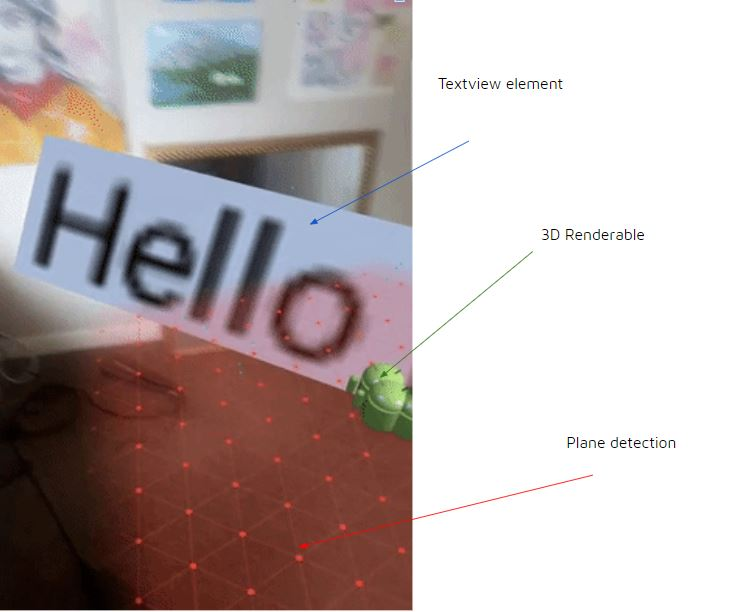
\includegraphics[width=1\textwidth]{images/sceneform_app.JPG}
\end{figure}



\subsubsection{Application Functionality}
\begin{itemize}
    \item Camera view can be moved around by the user to help find a plane.
    \begin{itemize}
        \item Triangulated mesh illustrates planes identified by plane detection algorithm.
    \end{itemize}
    
    \item On-tap listener captures user clicking area of the plane.
    
    \begin{itemize}
        \item Places an anchor and a renderable on tap location. Renderables are anchored once placed in the scene.
    \end{itemize}
    
    \item Device can be moved around and renderable with remain in place.

\end{itemize}
. 


\subsection{Shared AR with ARCore: Cloud Anchors}

Cloud anchors are Google’s approach to shared AR. Cloud anchors facilitate the creation of collaborative AR by sharing a common frame-of-reference, enabling multiple users to place virtual content in the same real-world location that can be seen on different devices in the same position and orientation relative to the environment[1]. 
\\
\\
Anchors are the fundamental element in ARCore. Anchors are estimates relating to a fixed location and orientation in the real world. Anchor poses are automatically adjusted by ARCore as its understanding of the environment improves based on the device's motion.
\\ \\
Cloud anchors are anchors that are assigned a unique ID and then uploaded to the ARCore Cloud anchor service. Once the anchor is hosted successfully the cloud anchor ID can be shared and resolved by other users. During this process, a new anchor with the original anchor's pose is assigned to the physical environment. The anchor’s pose is updated in real time on all devices accessing the cloud anchor.

The ARCore plugin for Android Studio provides support for developing applications with cloud anchors on Android devices. However, one of the key features in building a fully encompassing shared AR experience is creating an application that supports multiple platforms. For this reason, Unity in conjunction with the ARCore plugin was used to test the cloud anchor functionality. The ARCore plugin for Unity allows applications to be developed in a single codebase and then exported to both iOS and Android platforms. 

\subsubsection{Application Set Up}

\begin{itemize}
    \item A 3D Unity project was first created. In Unity’s Build Settings the target platform can be selected. For the purpose of this example, the Android platform was chosen but it should be noted iOS can also be selected for targeting Apple devices. 
    
    \item As directed in Google’s codelab demo \cite{arcore_codelab}, a basic AR scene was composed using ARCore’s First Person Camera prefab. To utilise ARCore’s environmental lighting feature, the Environmental Light prefab was also added to the Unity Scene.  Following this, a DetectedPlaneVisualizer prefab was included to illuminate the planes in the scene. 

    
    \item  With a basic application established, Cloud anchor functionality was then added. To use the ARCore Cloud Anchor API, an API key must first be obtained. Keys are available for free(limited usage) from the Google Cloud Platform. The key was added to the project via Unity’s Project Settings. The Cloud Anchor example scene provided in the ARCore package was then configured and added to the application. 
    
    
\end{itemize}

\begin{figure}[!ht]
\caption{ARCore Cloud Anchors Application}
\centering
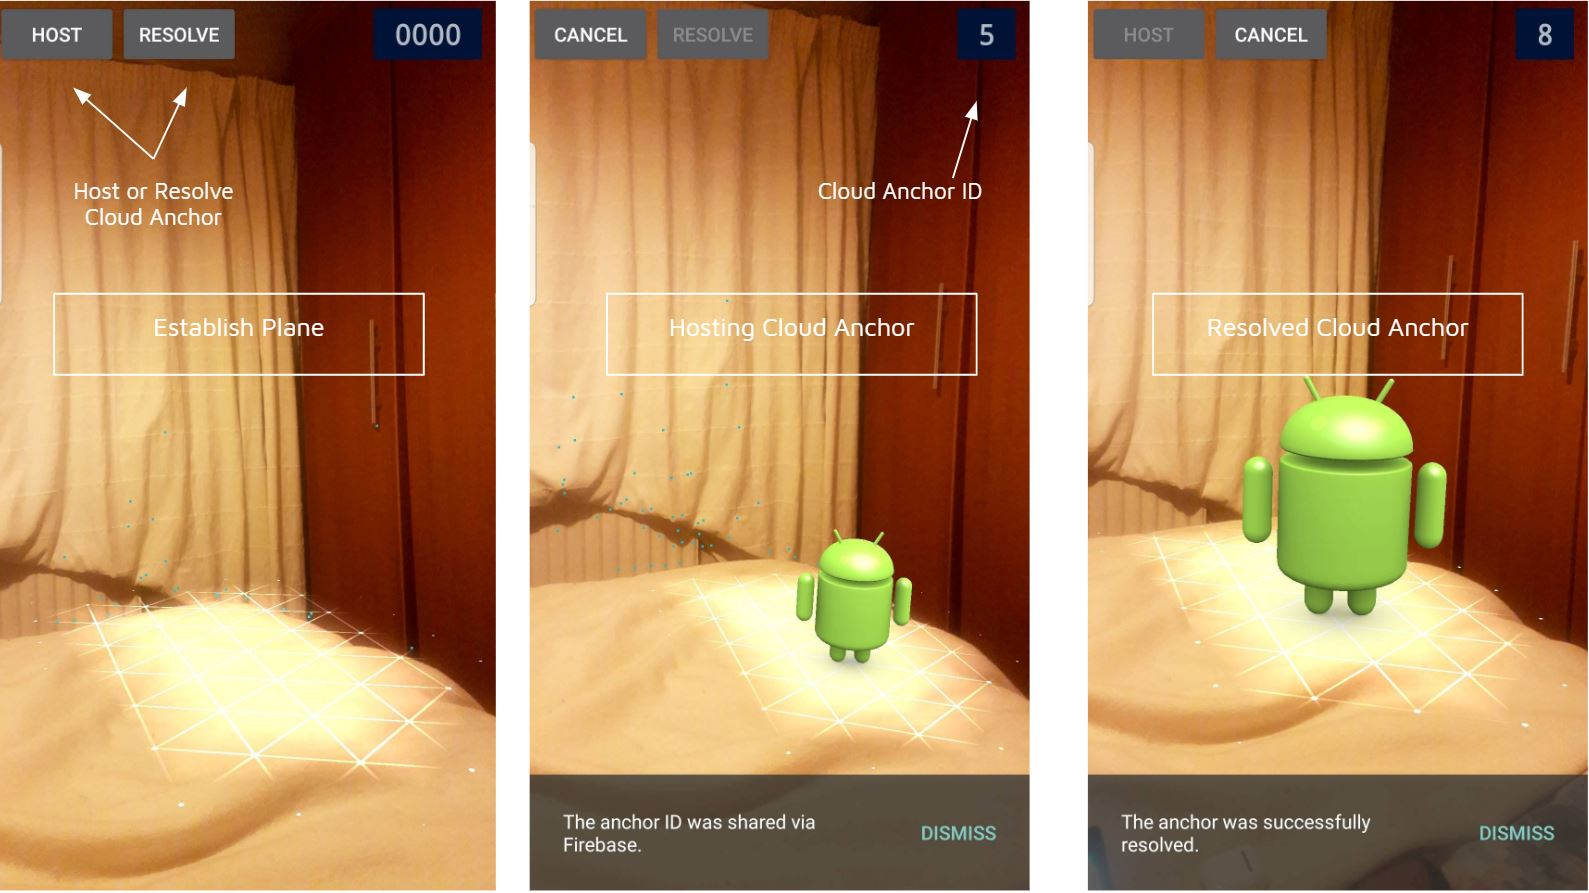
\includegraphics[width=1\textwidth]{images/cloud_anchors.JPG}
\end{figure}


\subsubsection{Application Functionality}

\begin{itemize}
    \item Camera can be moved around by the user to help find a plane. A Triangulated mesh illustrates planes identified by the plane detection algorithm.
    
    \item  On-tap listener captures user clicking an area of the plane. 
    
    \begin{itemize}
        \item Triggers the placement of an anchor and a renderable on tap location. Renderables are anchored once placed in the scene.
        \item Device can be moved around and renderable with remain in place.
    \end{itemize}
    
    \item A room number is created for the AR session(users may have multiple AR sessions).
A user wishing to join the AR Room can do so by entering a valid room number along with the user who hosted the room’s IP address. This is needed since any one user can create multiple rooms for the same physical environment.

\item The resolve button triggers a scan of the environment via the device’s camera. Distinct visual features are captured by the camera and uploaded to the cloud. The server tries to match these features with the spatial mapping of the host anchor.
If there is a successful match, the host anchor is loaded and placed in physical space. 
    
\end{itemize}

\subsubsection{ARCore Evaluation}
Creating a basic application using ARCore and Android Studio proved somewhat complex. While the initial documentation and code samples provided by Google are helpful and informative - moving away from these and trying to implement a custom application required a considerable amount of tweaking and changing small elements in various areas of code. For this reason, the learning curve associated with developing Android applications with ARCore could be considered quite high. However, this gives the developer a fine degree of control over the AR scene created, along with a range of options for customizability.

ARCore’s support for shared AR is straightforward to implement. The adoption of Unity to create cross-platform applications using the ARCore plugin was found to significantly expedite the development process. ARCore’s helper assets and configurable prefabs are clear and simple, allowing the quick assembly and implementation of a shared AR experience.  
Furthermore, the cloud anchor system proved robust when tested with multiple devices and AR sessions. 

In terms of suitability for this full stack application, ARCore and Unity lacked the key features required for this project. Unity is a game development platform, and as a result, the nature of its functionality and features are based on game development. Creating elements core to a complete mobile application, such as the user interface, navigation and database management is complex and cumbersome with Unity, as these elements are not the focus of the platform. To combat this, the insertion of a Unity ‘view’ into a framework that handles UI components such as Ionic was explored. However, this proved unsuitable as it was extremely taxing on the mobile device’s CPU, resulting in unstable and erratic behaviour within the application. 


\subsection{Wikitude}
The Wikitude SDK is a software library and framework for mobile applications used to create augmented reality experiences. The SDK supports location-based augmented reality, along with image recognition and tracking based augmented reality \cite{wikitude_docs}.


\begin{figure}[!ht]
\caption{Wikitude Architecture \cite{wikitude_docs}}
\centering
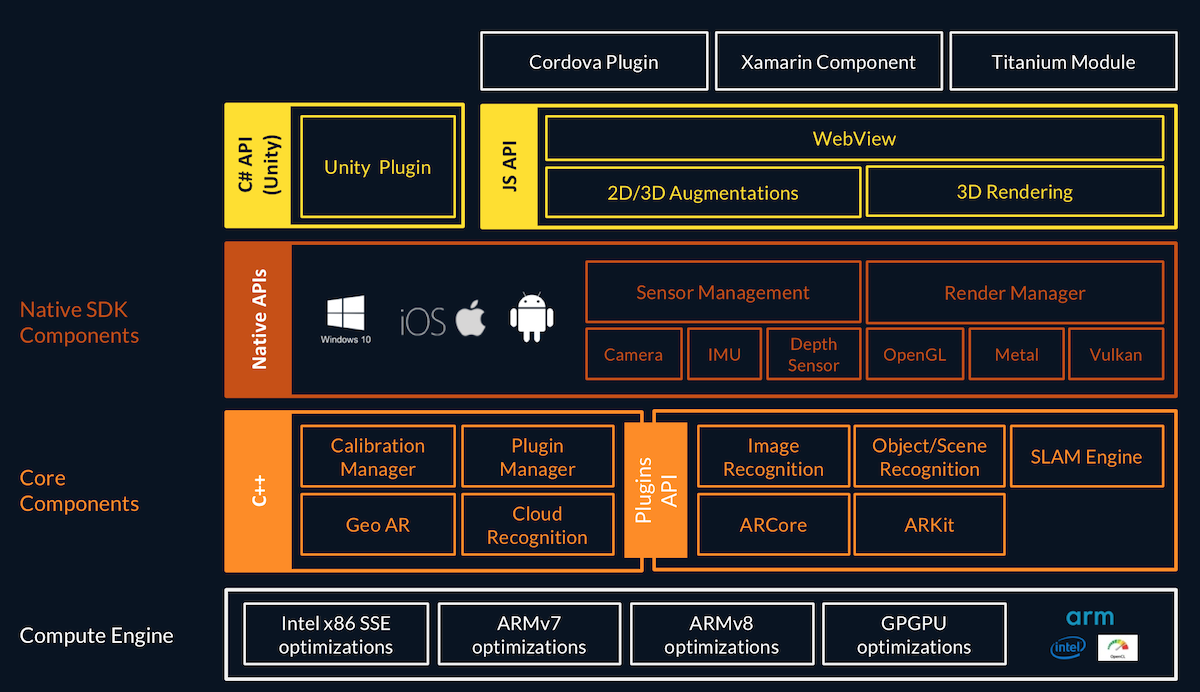
\includegraphics[width=1\textwidth]{images/wikitude_architecture.png}
\end{figure}

The image above shows the different components of the Wikitude SDK. Wikitude allows for the creation of augmented reality apps in a myriad of development environments and platforms. Platforms and extensions currently supported by Wikitude include Android, iOS,  Cordova, Titanium, Xamarin, Unity, Epson Moverio smart glasses and Vuzix

\subsubsection{ARchitect World}
The Wikitude SDK leverages web technologies to allow the creation of cross-platform augmented reality experiences. These augmented reality experiences are called ARchitect worlds. ARchitect worlds are HTML pages that can utilize the ARchitect API to generate objects in augmented reality.

The core concept is to insert an architectView to the project, (usually, a file named [projectname].html located in ./assets directory)and then notify it about lifecycle events. The architectView creates a camera surface and handles sensor events such as user tap, click or drag motions. The experiences are written in HTML and JavaScript and call methods in Wikitude's AR-namespace (e.g. AR.InstantTracking).

\subsubsection{SLAM}
SLAM (Simultaneous Localization and Mapping) is a computer vision technology that creates an understanding of the physical world through the use of feature points \cite{slam}. SLAM uses only visual inputs to perform location and mapping, meaning that the only sensor required is a camera. A feature point map is constructed and continuously updated. The agent’s location within this map is simultaneously recorded and tweaked as the understanding of environment evolves.  Wikitude provides SLAM technology via its Instant Tracking feature.

\subsubsection{Instant Tracking}
Instant Tracking is the principal algorithm that provides tracking functionality in the Wikitude SDK. The algorithm has two primary phases, the Initialization State and the Tracking State. 
\\ \\
During the initialization state, the height of the users’ device is provided in order to accurately adjust the scale of augmentations within the scene.  The tracking device height is described by the developer before run-time. The user is required to point the device so that the alignment indicator is in a stable position. Once the alignment is found to be satisfactory (the users must actively confirm), the ground plane for the AR scene is established. 

\begin{figure}[!ht]
\caption{Wikitude Instant Tracking }
\centering
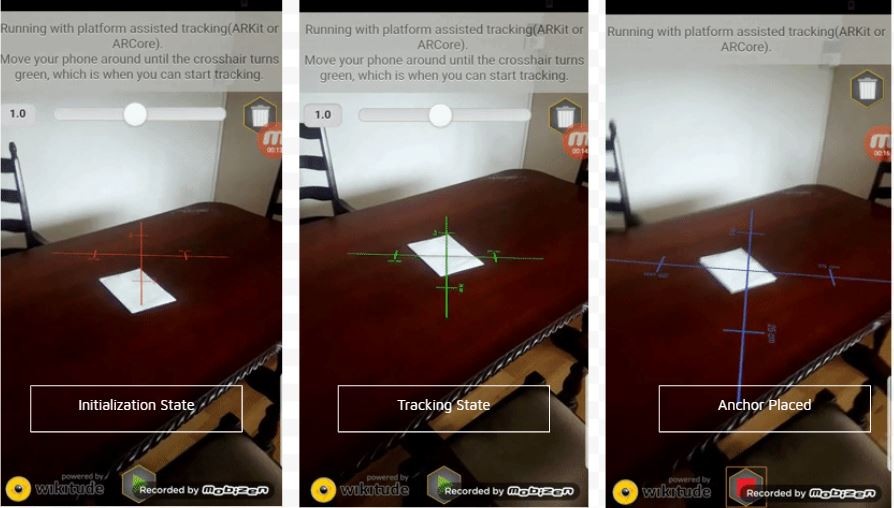
\includegraphics[width=1\textwidth]{images/wikitude_tracking.JPG}
\end{figure}

The tracking state commences once the plane has successfully been established.  In this state, the environment is being tracked continuously, which allows for augmentations to be placed within the scene.

\subsubsection{Instant Tracking Implementation}
Wikitude provides access to the instant tracking algorithm via two classes, AR.InstantTracker and AR.InstantTrackable. 

\subsubsection{Instant Tracker}
An InstantTracker represents an instance of the instant tracking algorithm. It does not require any pre-existing target information and so, can immediately start tracking. Minimally, It can be instantiated without any parameters in the following manner: 


\begin{minted}
[
baselinestretch=1.2,
fontsize=\footnotesize,
linenos
]
{javascript}

 this.tracker = new AR.InstantTracker();
\end{minted}

To ensure the most accurate tracking information, it is ordinarily instantiated with the device height. The onChangedStateFn() callback function allows the developer to invoke functionality when the tracking algorithm changes state (from initializing to tracking).

\begin{minted}
[
baselinestretch=1.2,
fontsize=\footnotesize,
linenos
]
{javascript}

this.tracker = new AR.InstantTracker({
    onChangedState:  function onChangedStateFn(state) {
        // react to a change in tracking state here
    },
    // device height needs to be as accurate as possible to have an accurate scale
    // returned by the Wikitude SDK
    deviceHeight: 1.0,

 // The initial orientation at which the instant tracking plane should be displayed in degrees.
 // Default value is AR.CONST.INITIAL_INSTANT_TRACKING_PLANE_ORIENTATION.HORIZONTAL (0°).
    trackingPlaneOrientation: 45.0
});

\end{minted}
\caption{\cite{instant_tracking}}

\subsubsection{Instant Trackable}
The InstantTrackable Class describes a virtual object attached to an InstantTracker. Drawable augmentations can be bound to an instance of InstantTrackable, allowing them to receive relevant transformations during the tracking state. An InstantTrackable may also take the form of a tracking plane. Triggers can be connected with InstantTrackers to invoke events and functions to react to changes in the tracking state.  \\ \\
To create an instance of the InstantTrackable Class, an InstantTracker object must be passed as a parameter to its constructor. 

\begin{minted}
[
baselinestretch=1.2,
fontsize=\footnotesize,
linenos
]
{javascript}

this.instantTrackable = new AR.InstantTrackable(this.tracker, {
    drawables: {
        cam: aDrawable,
        initialization: anotherDrawable
    },
    onTrackingStarted: function onTrackingStartedFn() {
        // do something when tracking is started (recognized)
    },
    onTrackingStopped: function onTrackingStoppedFn() {
        // do something when tracking is stopped (lost)
    }
});


\end{minted}
\caption{\cite{instant_tracking}}

\subsubsection{SMART - Seamless AR Tracking}
SMART is an API which integrates ARKit, ARCore and Wikitude's SLAM to provide multi-platform sugmented reality tracking. The goal of SMART is to ensure the most accurate AR tracking for the device in use. The SMART API checks the platform of the device. If it is identified as an Android device, it then checks whether it is supported by ARCore, if so - it loads ARCore’s methods for improved tracking. Similarily, if the device runs iOS, ARKit’s tracking algorithms are used. If the device is not supported by either ARcore or ARKit - Wikitude's SLAM/basic Instant tracking algorithm is used. 

SMART is enabled by default but can be disabled by setting a parameter when creating an AR.InstantTracker with the smartEnabled option. The behaviour cannot be changed during runtime.

\begin{minted}
[
baselinestretch=1.2,
fontsize=\footnotesize,
linenos
]
{javascript}

new AR.InstantTracker({
    smartEnabled: false
});

\end{minted}
\caption{\cite{instant_tracking}}


SMART provides improved tracking capabilities at the expense of control. Therefore, some of Wikitude’s features are not available when platform tracking capabilities are used by enabling SMART. The following figure illustrates the functionality available with SMART tracking activated. 

\begin{figure}[!ht]
\caption{SMART Compatibility}
\centering
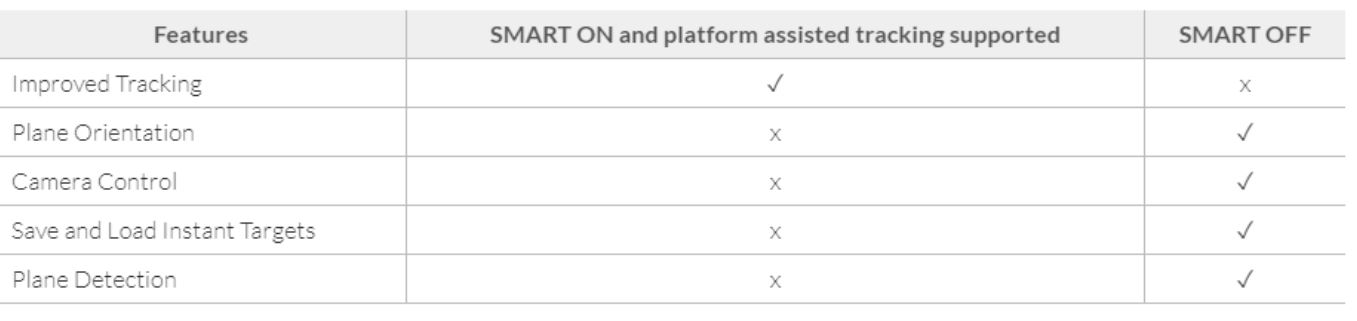
\includegraphics[width=1\textwidth]{images/smart.JPG}
\end{figure}

\subsubsection{Object and Scene Recognition}
Object Recognition and Tracking let you detect objects and entire scenes that are pre-defined by the developer. The scene and object recognition feature is based on Wikitude's SLAM engine, which is used throughout the SDK for environment tracking. The object recognition feature tries to find and match a pre-created reference in the live camera image. This pre-created reference is called  an Object Target. Object Targets can be created using videos or images as source material. The source material is converted into a Wikitude Object Target Collection, which is stored as .wto file \cite{wikitude_docs}. Wikitude’s studio Manager is a free web tool that helps manage and create object targets. 

\subsection{Augmenting 3D Content}
\subsubsection{AR.Model}
The AR.Model class represents a drawable AR object as a 3D model. The Model type consists of a link to a .WT3 file that has been created using the Wikitude Encoder. During a model’s instantiation, setup parameters can be provided to allow for customization of its properties, for example, the model’s scale and rotation. 
\\ \\
The following example illustrates the initialization of a Wikitude Model
\begin{minted}
[
baselinestretch=1.2,
fontsize=\footnotesize,
linenos
]
{javascript}

//create a new Model and pass some setup parameters
var model = new AR.Model("models/my3dModel.wt3", {
  // scales it to half of the original size
  scale: {
    x: 0.5,
    y: 0.5,
    z: 0.5
  },
  // rotates it 90 degrees around the z-axis and 180 degrees around the x-axis
  rotate: {
    x: 180.0,
    y: 0.0,
    z: 90.0
  },
  // moves the 0bject 5 SDUs along the x- and the y-axis
  translate: {
    x: 5,
    y: 5,
    z: 0
  },
  onClick : function() {
    //something happens
  }
}
\end{minted}
\caption{\cite{instant_tracking}}


\subsection{Shared AR with Wikitude: Persistent Targets}
The Wikitude SDK  does not officially support functionality for Shared AR. However, as the SDK uses JSON objects to build AR experiences, the Persistent Instant Targets feature has emerged as a manner of exploiting this to dynamically save and load AR experiences. By essentially saving and loading a stringified JSON object representing the AR scene, it is possible to create shared AR that may be persistently accessed by multiple users across devices and operating systems. 


\subsubsection{Save Instant Target}
To save an AR experience, an active InstantTracker in the tracking state must be present in the ARchitect world. The Save Instant Targets functionality calls on the AR.platform.sendJSONObject method to send the current AR scene as a JSON object to the platform.  
\begin{minted}
[
baselinestretch=1.2,
fontsize=\footnotesize,
linenos
]
{javascript}

 if (this.tracker.state === AR.InstantTrackerState.TRACKING) {
        AR.platform.sendJSONObject({
            action: "save_current_instant_target",
            augmentations: JSON.stringify(augmentations)
        });
    }
    
\end{minted}
\caption{\cite{instant_tracking}}
The AR scene’s current models, scaling, rotations and positioning are bundled into an the augmentations object and sent from the ARchitect world to the platform.

\subsubsection{Load Instant Target}
In order to load an instant target, a path to a valid JSON object representing an AR scene’s augmentations must be provided. Similar to the process of saving an AR scene, to load one, AR.platform.sendJSONObject and architectView.callJavaScript are used. 

\begin{minted}
[
baselinestretch=1.2,
fontsize=\footnotesize,
linenos
]
{javascript}
// Inform the platform code to load a AR scene
loadExistingInstantTarget: function () {
    AR.platform.sendJSONObject({
	// triggers this method on the platform side code
        action: "load_existing_instant_target"
    });
}
\end{minted}
\caption{\cite{instant_tracking}}

The platform code receives the call to load an AR scene and proceeds to do so in a manner custom to the application. For example, the augmentation may be loaded from a local file on the device or a remote database. 

\subsubsection{Wikitude Evaluation}
Creating applications utilising the Wikitude SDK has numerous benefits. As the SDK is based on web technologies, it leverages significant flexibility. This is evident in the diverse platforms it currently supports. Furthermore, Wikitude’s SMART API provides support for 92.6\% of iOS devices and roughly 35\% of Android devices available on the market\cite{instant_tracking}. In contrast, ARCore currently only supports 28.2 percent of Android devices currently available \cite{android_stat}.

Documentation and support for shared AR with Wikitude is lacking in comparison to that of ARCore. Nevertheless, the underlying technology remains open to develop and build upon. Although this is more work for the developer, it yields greater control and autonomy over its implementation. 

While ARCore may be considered more robust as its underlying codebase is developed in C\#, Wikitude’s use of Javascript and JSON promote rapid development when utilising the SDK. Additionally, Wikitude can be easily integrated with a wide range of technologies in the development of a full-stack application. For example, the SDK can be used in conjunction with platforms such as Ionic and Apache Cordova to create cross-platform applications. 

Given its use of web-based technologies and wide range of supported devices, Wikitude's SDK was deemed most suited to this projects goal of creating a full stack, cross platform application.


\chapter{Methodology}

\section{Project Management}
The following section outlines the processes undertaken during the various stages of the project’s planning and development. It also describes the manner in which decisions regarding design and implementation were conducted. 

\subsection{Brainstorming}
The first stage of the project involved an exploration of the latest advancements in the software development domain. In the search for a viable project idea, themes such as artificial intelligence, Internet of Things, virtual reality and augmented reality were investigated and considered. During this phase, both news and scholarly articles were reviewed to identify trends and growing areas pertinent to the computing field. Following that, a base of possible topics fitting the criteria for this Applied Project \& Minor dissertation was compiled. With the guidance of my supervisor, the topic that piqued the interest the was selected - AR. 

Following determining the area of interest, a period was spent establishing the state of the field in Augmented Reality. The primary method employed to grasp a sense of the possibilities available was reading and documenting the latest advancements relating to AR.


\subsection{Agile}
Given the changing nature of this research-heavy project, employing Agile methodologies was crucial to facilitate an effective development cycle.

Initially, a period was spent researching the most effective software development methodology. Given the changeability of a research-based project, a Waterfall model with meticulous planning was immediately ruled out. It was concluded an Agile Method would be most appropriate. Choosing which Agile methodology to employ provoked further research. Literature indicates that there is a lack of statistical evidence relating to whether a Scrum or Kanban approach is most effective\cite{sugimori1977toyota}. For this reason, a combination of Kanban and Scum methodologies were applied to implement Agile Development. Given it was just one developer working on this project, the luxury of creating a developer specific workflow was exercised. Various elements from the outlined Agile methodologies were combined, to create a custom project planning and software development method.

\subsubsection{Kanban}
The Kanban methodology was implemented throughout the project development. To facilitate the creation and management of storyboards, Trello was used. A board was created with three stages - \say{To Do}, \say{In Progress}, \say{Done}. Tasks representing the project’s critical path were added as cards via Trello’s user interface.

\begin{figure}[!ht]
\caption{Trello Storyboard}
\centering
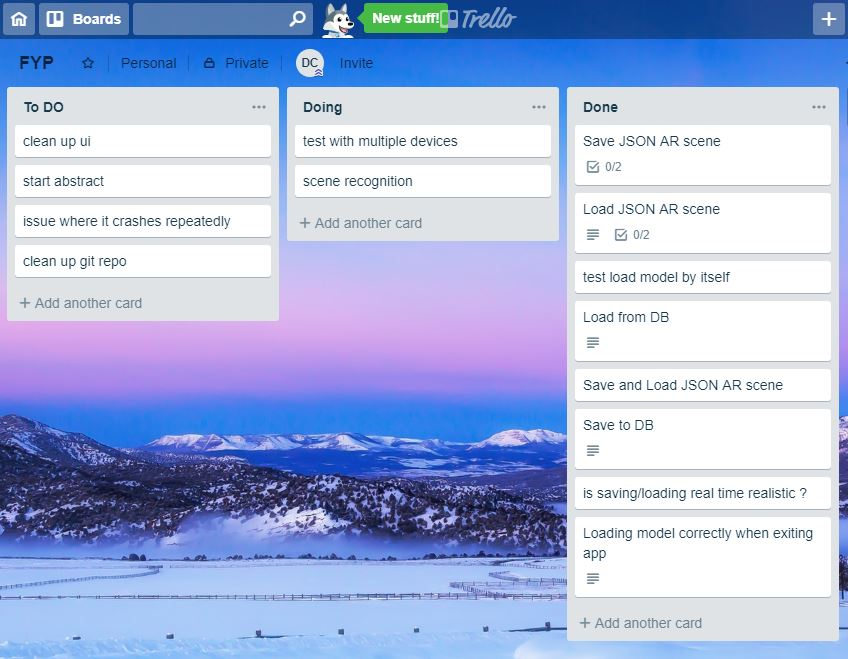
\includegraphics[width=1\textwidth]{images/trello.JPG}
\end{figure}

\subsubsection{SCRUM}
In conjunction with Kanban, the Scrum methodology was executed. In this project, sprints were one week in length. At the end of each week, a meeting took place between developer and supervisor. During this time progress from the sprint was discussed along with any ‘blockers’(hindrances to project development). Goals for the next sprint were also established and logged in the GitHub readme following these meetings. 


\section{Version Control}
\subsection{Github}
Github was used as the method of version control in this project. A remote Git repository was created on Github. During development, code was tracked using git and then uploaded to this repo. Github provided two primary functions for development, tracking code changes and also the security of having the code base backed up in case of any issues on my local machine. Sprint planning was also logged on the github readme.  


\section{Literature Review}
To gather relevant literature sources, science and computing databases (ScienceDirect, Omni File Full, Mega text, Science Citation Index) were queried. To gather information pertaining to AR technologies, databases were queried for the strings ”augmented reality” AND ”state of the field” OR ”state of the art”. To find resources relating to augmented reality in the context of architecture, the strings ”augmented reality” AND ”architecture” OR ”architectural” were queried. Previous literature [3], highlights that there is a lack of consistency in both academic and professional fields when discussing augmented reality as it is often used interchangeably with other mixed reality technologies. To combat this, the NOT operator was used on the term ”virtual reality” as this review solely examines the application of augmented reality technologies. In cases specific to outlining current technologies, such as software development toolkits, developer documentation from internet sources are referenced.

The topic was expanded upon by researching databases for articles and publications on the topic. However, given that the area itself is considered ‘bleeding edge’, informative resources proved scarce. It was found to be more effective to investigate documentation relating to current AR SDKs and review whether they featured the required functionality to implement shared AR. This documentation was also used to understand the various processes behind building collaborative AR experiences.  While this stage initially presented itself as quite challenging due to the limited resources available relating to the topic, it manifested as an exciting opportunity to make a contribution to shared AR’s limited body of research.

\section{Testing}
\subsection{Web Application Testing}
Selenium was chosen as the method of testing the system's web application. Having had previous experience with the Selenium IDE, it was for this reason it was selected as a testing method.
\subsection{Augmented Reality Testing}
Sourcing a method of testing the augmented reality aspect of mobile application proved challenging at first. However, it was eventually decided that testing the robustness of the application's plane detection and tracking would be beneficial. This was achieved by attempting to place an AR trackable in a selection of contrasting lighting conditions and evaluating the effectiveness and speed of the plane detection. 




\section{System Architecture}
The system is comprised of three primary components:
\begin{itemize}
    \item Ionic AR Mobile application
    \item Firebase NO-SQL database
    \item Ionic Web Application
\end{itemize}


\begin{figure}[!ht]
\caption{System Architecture}
\centering
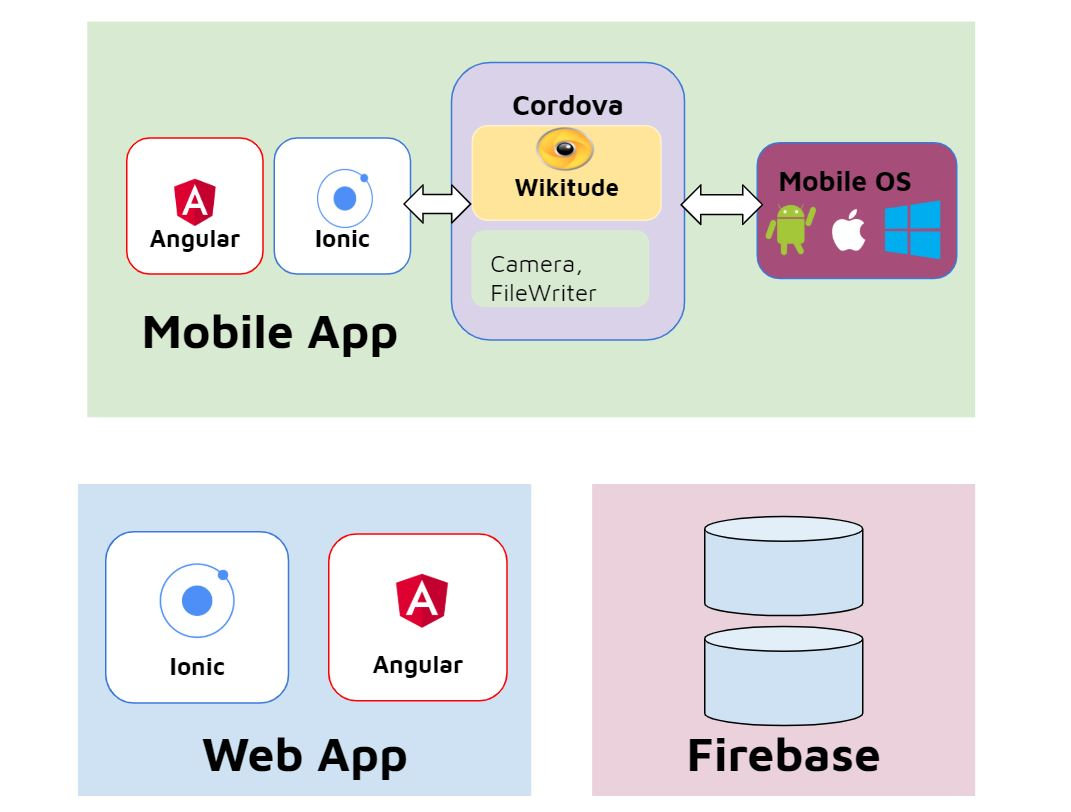
\includegraphics[scale=0.5]{images/sys_architecture.JPG}
\end{figure}


\subsection{Ionic Framework}
In conjunction with Apache Cordova, the mobile application was built using Ionic 3. Ionic was selected because it supports the creation of cross-platform applications through the use of web technologies. Additionally, it integrates with Apache Cordova, which includes a plugin for the Wikitude SDK. Ionic handles the front-end side of this application, i.e the components that comprise the User Interface, while Apache Cordova provides plugins and support or access to the hardware of the native device. 

\subsection{Wikitude Cordova plugin}
The Wikitude Apache Cordova plugin was used to add Wikitude’s functionality to the mobile application. To include it in the project, the following command was executed using the ionic CLI tool. 
\begin{minted}
[
baselinestretch=1.2,
fontsize=\footnotesize,
linenos
]
{java}
ionic cordova plugin add https://github.com/Wikitude/wikitude-cordova-plugin.git

\end{minted}


\subsection{Firebase}
Firebase was chosen as the database for the project because of its support for applications built using web technologies. NPM was used to install the firebase plugin.

\begin{minted}
[
baselinestretch=1.2,
fontsize=\footnotesize,
linenos
]
{java}
npm install --save firebase
\end{minted}



An API key is required to use firebase. This was obtained by accessing the Firebase Console via the Google Cloud Platform. With the application registered and configured, the firebase credentials were then added to the Ionic Application in the firebase.credentails.ts file.

Firebase’s real-time database is used to facilitate Shared AR within the application. A reference to the database was created within the application. Following this, a listener was added to the database reference. This allows the application to be automatically notified of any changes to the database. 

\begin{minted}
[
baselinestretch=1.2,
fontsize=\footnotesize,
linenos
]
{javascript}
// create databse refernce
        var ref = firebase.database().ref('/ARSessions/');

             // getting the latest data from the db
              this.ref.on('value', snapshot => {
                dbres = snapshot.val();
              });

\end{minted}

In the context of this mobile application and shared AR, this functionality is used to update the user’s AR scene in real time in the event of changes made to it by another user. In this manner, all users are in sync - viewing and interacting with the same ar scene loaded via the same database reference.



\chapter{System Design}
The system is composed of three primary components, a cross-platform mobile application for viewing and sharing architectural models using AR, a database for storing augmented reality models and sessions and finally, a CRUD web application for managing and uploading models to the database. 

\section{Database}
For the purpose of this project, Firebase was used to store and sync data. The reason it was selected was for its NO-SQL, real-time data synchronization - a feature key to implementing shared AR. 

\subsection{Cloud Firestore}
Firestore is used to host and store the architectural models used in the application. The web client accesses firestore to create, read, update and delete these models. Models can be uploaded to the database using the uploadToStorage function provided by the Firebase plugin. 

\begin{minted}
[
baselinestretch=1.2,
fontsize=\footnotesize,
linenos
]
{java}
  // send file and name to data store
    let upload = this.dataProvider.uploadToStorage(text, file);

\end{minted}

\subsection{Realtime Database}
FIrebase’s real-time database is used to store data pertinent to the mobile application. The application’s database has two primary data stores - one for storing  AR sessions and another for storing the URLs that point to the architectural models located in the cloud firestore databse.

\begin{figure}[ht!]
\caption{Database Schema}
\centering
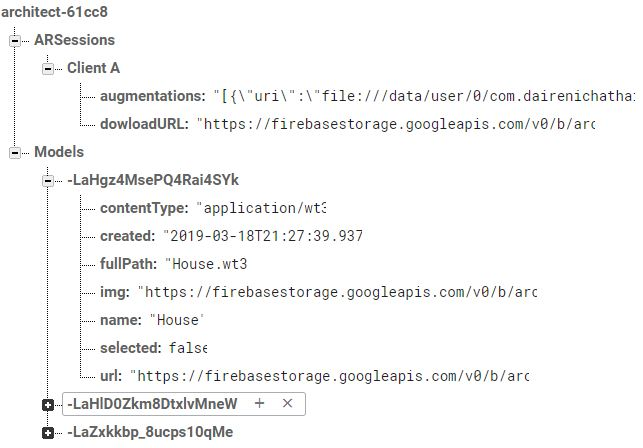
\includegraphics[scale=0.55]{images/firebase_databse.JPG}
\end{figure}


\section{Web Application}
The web application functions as a tool for managing the architectural models used in the mobile application. In a real-world use case, the architect or product owner would have access to the web client, and from here, could organise the models they wish to share with customers. 

The web app leverages Firebase’s Cloud Firestore database to host the models, which take the form of .wt3 files. The user interface facilitates full CRUD behaviour, allowing the user to create, read, update and delete any files located in the application’s database.

The web client is a single page application built using the Ionic framework. The root page of the application presents all the .wt3 files currently stored in the database.

\begin{figure}[ht!]
\caption{Web Application}
\centering
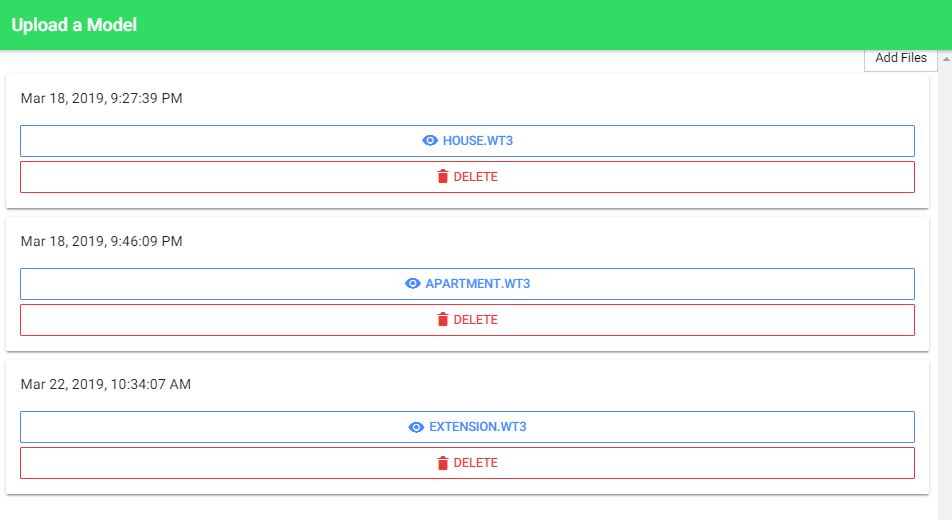
\includegraphics[width=1\textwidth]{images/web_client.JPG}
\end{figure}


\begin{itemize}
    \item The Add Files button utilises the Apache Cordova file picker plugin to allow the user to select a local file to upload.
    
    \item Clicking a the files triggers an instant download to the user’s device. This feature can be used to preview a model on the user’s local device. 

    \item The delete button removes the file from the database. A popover confirms the successful deletion of a file. \\ \\
\end{itemize}



\section{Mobile Application}

The objective of the mobile application is to provide the user with a tool to preview architectural models through the use of augmented reality. 

An example use case would be an architect and customers discussing and designing plans for a new construction. As illustrated by \cite{lorensen1987marching}, people often find it difficult to visualize 3D models in physical space without sufficient visual aids. This mobile application would serve to aid architects in expressing their designs to customers. The architect creates a session that clients can join. In this session, an architectural model can be shared between parties, enabling multiple users to interact with virtual content in the same real-world location that can be seen on different devices, in the same position and orientation relative to the environment. This way, the proposed model can be viewed and interacted with, promoting a collaboration and a common understanding between users. 


\subsection{Home Page}

This is the root page of the application. From here the user may proceed with one of the following options, creating a new AR Session or loading a previously saved session. These options are presented in the form of two buttons.

\begin{figure}[ht!]
\caption{Home Page}
\centering
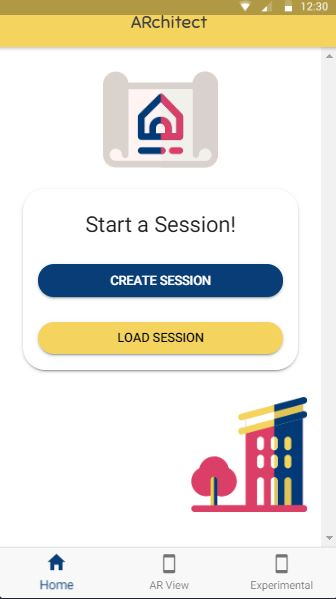
\includegraphics[scale=0.65]{images/home_page.JPG}
\end{figure}


\begin{itemize}
    \item Selecting the \say{Create Session} button triggers navigation to the \say{Create Session Page}.
    
    \item Selecting the \say{Load Session} button triggers the Load Session Popover. 

\end{itemize}



\subsubsection{Load Session Popover}
The Load Session popover features a single input field to allow the user to enter a session name. 


\begin{figure}[ht!]
\caption{Load Session Popover}
\centering
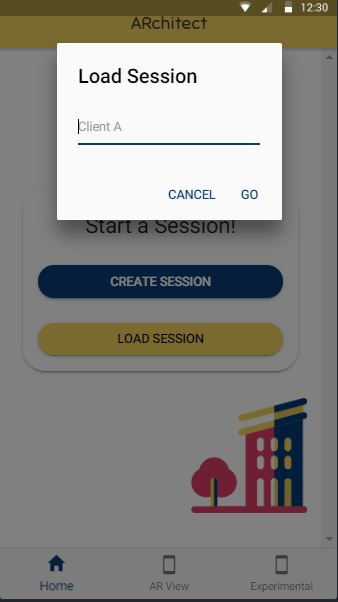
\includegraphics[scale=0.55]{images/load_session_popover.JPG}
\end{figure}

\begin{itemize}
    \item The \say{Go} button then checks the database for any AR sessions with a matching name. If it fails to find a match, a popup is used to inform the user.
    
    \item If a match is found, the AR session is loaded from the database and written device file system. 
    
    \item
    The model required in the AR session is written to a .wt3 file on the file system.

    \item
    Once all the required resources are loaded from the database, the user is navigated to the \say{AR} View page. \\ \\
    
    
\end{itemize}



\subsection{Create AR Session Page}
On this page, the user is presented with an input form to provide details for the creation of a new AR Session.

\begin{figure}[!ht]
\caption{Create AR Session Page}
\centering
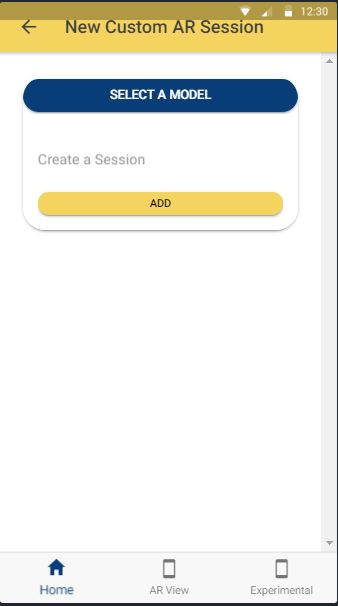
\includegraphics[scale=0.55]{images/create_session_page.JPG}
\end{figure}

\begin{itemize}

    \item The \say{Select a model} button opens a modal displaying architectural models that can be selected to use in the shared AR session. Model information is dynamically loaded from the database. The model information contains the model title, thumbnail image and a URL to the storage location of the .wtc file in the database. 

    \item The input field allows the user to specify a name for the session. This name becomes the session key which can be shared with other users wishing to engage in the same AR session.
    
    \item The \say{Add button} triggers the creation of the AR session. An entry is made in the database using the session name as an object key. The selected model is then downloaded using the model URL and written locally to the device storage. 

    
\end{itemize}


\subsection{AR View}
This page is used to present the AR content. The ARchitect world is initialized so that augmented content can be rendered.

\begin{figure}[!ht]
\caption{ARView Page}
\centering
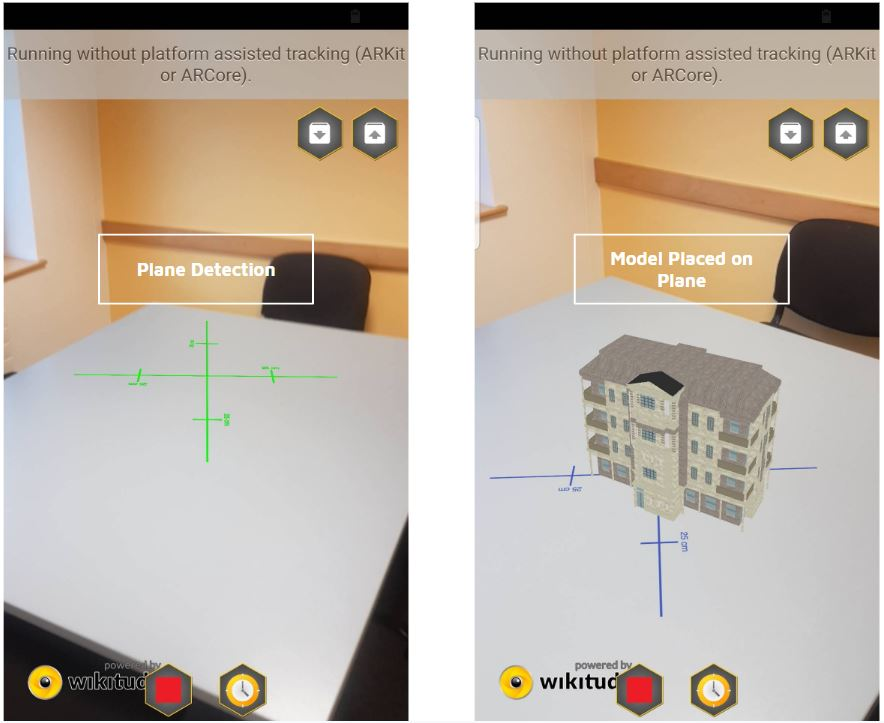
\includegraphics[scale=0.55]{images/arview_page.JPG}
\end{figure}

\begin{itemize}
    \item To place a model within the scene the user must first detect a plane. The cross-hair drawable is used to aid the user in detecting a plane. 

    \item The slider can be used to adjust the cross-hair size so that the plane can be scaled up or down depending on the users preference. 
    
    \item Once a valid plane is identified, the cross-hair changes from red to green. The user must then tap to anchor the plane. The user can then place a model on the plane by tapping the area they wish to plant it.
    
    \item The user can interact with the model via a drag gesture to move it or pinching to scale. The model can also be rotated with a select and drag gesture.
    
    \item Any alterations made to the model are updated to the database in real-time. Any other users connected to the same session will see the updates made to model. 


\end{itemize}


\subsection{Experimental Page}
 This page serves to highlight Wikitude's Scene Detection Functionality. 
 \begin{itemize}
     \item The camera can be used to scan the environment for a predefined Object Trackable(scene). 
     \item Once the scene is recognised, an architectural model is placed within the scene, using the model's specified scale, rotation and orientation.
 \end{itemize}



\subsection{Scene Detection}
Scene detection is implemented using Wikitude's Object Recognition and Scene Detection functionality. An object tracker was created using Wikitude Studio. This was achieved by uploading a selection of images representing the area to be recognised. Wikitude Studio was then used to place a model within the defined area. Following this, the tool generates the .wto (Wikitude Object Trackable file). This file was then added to mobile application. The  \say{Experimental Page} within the app illustrates Scene Recognition in action. 

\subsection{Shared AR}
Shared AR is implemented using Wikitude's Persistent Tracking functionality. To create a shared AR session, a unique session key must be provided by the user. Following this, an entry is created in the \say{ARSessions} object in the database. Once an instance of an InstantTrackable is in the tracking state and a model is associated with it, the database begins listening for updates to the AR scene. 
\\  
The user can interact with the AR scene via altering the model’s scale, rotation and orientation. Any changes in the AR session trigger an update in the database. These changes are propagated to all other users interacting with the same AR session. In a similar way, if another user creates a change in the scene, the current user’s AR scene will be updated to reflect it. Firebase’s real-time database is used to facilitate the live syncing of ar scenes. 
\\  \\
When loading the AR Scene, its JSON representation is pulled from the database and written to a file locally. The writing of this file is achieved through the use of the Apache Cordova File plugin.


\begin{minted}
[
baselinestretch=1.2,
fontsize=\footnotesize,
linenos
]
{javascript}
// get access to file system
    window.resolveLocalFileSystemURL(cordova.file.externalDataDirectory, function(fs) {
        // get the file, if it doesn’t exist, create it
        fs.getFile("SavedAugmentations.json",
          { create: true, exclusive: false },
          function(fileEntry) {
            // instantiate the writer
            fileEntry.createWriter(function(writer) {
            // write the augmentation json object loaded from DB
              writer.write(augmentations);
            }
          }
              }

\end{minted}

An instance of the FileWriter Object is created. The augmentations loaded from the database are then written to the SavedAugmentations.json file. Due to security restrictions on Android Devices, the device’s external data directory is the only directory used for reading and writing content within the application. 


\chapter{System Evaluation}
The general goal of this project was to evaluate and establish the current tools available for creating cross-platform, multi-user augmented reality mobile applications. More precisely, the project’s objectives can be described as follows:
\begin{itemize}
    \item Evaluate and establish the current tools available for creating cross-platform multi-user augmented reality mobile applications.
     \item Implement shared augmented reality.
    \item Build a full stack system for use in architecture, featuring shared augmented reality technology. 

\end{itemize}
\section{Evaluation of Objectives}
The following section outlines how the objectives described above were implemented in the completed system.

\begin{itemize}
    \item \textit{Evaluate and establish the current tools available for creating cross-platform multi-user augmented reality mobile applications}. During the research phase of the project, SDKs known to have the functionality required to facilitate shared AR were investigated. Each of the selected SDKs were thoroughly reviewed. Relevant literature pertaining to the SDK was gathered and examined. Additionally, sample applications were created to accurately evaluate the advantages and limitations of each SDK. 
    
    \item \textit{Implement Shared Augmented Reality}. Shared augmented reality was successfully implemented in this system using the Wikitude SDK. Multiple users can share and interact with architectural models in a synchronized augmented space. While this initially proved a difficult task as Wikitude does not provide complete support for this functionality, it was successfully implemented in the mobile application.
    
    \item \textit{Build a full stack system for use in architecture, featuring shared augmented reality technology}. The final system created successfully achieves this objective. Architectural models can be interacted with using the mobile application developed. The application features a UI, cross-platform middle-ware and Firebase as a back-end. In addition to this, extra functionality was added to the application. A web application was added during the development phase to facilitate the management of AR assets within the mobile application. This feature was included as it serves to illustrate how the mobile application’s data can be managed in production environment. Additionally, Wikitude's Scene detection and recognition features were implemented. The reason for their addition was to add further value to the application’s use in architecture. Viewing how an architectural model superimposed on the area of its intended development is significantly useful for both architects and their clients. 
    
\end{itemize}

\section{Opportunities for Improvement}
While the proposed objectives for this project were achieved, there are, undoubtedly, areas in which the overall system can be improved upon.

\subsection{Testing}
Although basic tests usability tests were conducted on the system, the application lacks sufficient testing. To ensure a more robust mobile application, unit testing using Karma and Jasmine would ideally be employed. Furthermore, extracting quantifiable metrics also proved challenging while testing the system. Given the nature of augmented reality technology, it proved difficult to source a means of quantitive testing. 

\subsection{Authentication \& Security}
The mobile application and web application lack functionality for user authentication. While user authentication was never in the scope of this project, it is a critical feature needed to make the system production-ready.

\subsection{Mobile Application Crashes}
 A period of testing revealed that occasionally, the mobile application is prone to crashing. In an attempt to resolve this issue, time was spent utilising debugging tools and investigating logs to identify the source issue. Unfortunately, the issue remains unresolved. Given the limited time scale, and while also in keeping with the spirit of the Agile methodology, it proved more effective to continue with the development of features on the project’s critical path as the bug was not deemed severe.




\chapter{Conclusion}
This project sought to investigate and demonstrate the various methods and technologies currently used to create shared augmented reality experiences. As illustrated in section 5.1, while the end goals of the project were indeed achieved, the wealth of knowledge obtained during the process of its development can be considered the most valuable outcome of the project. 

During the research phase of this project, scholarly papers relating to shared augmented reality showed to be extremely scarce. Examining the tools for shared augmented reality creation is a novel concept and therefore an area in which research is particularly valued in the academic community. Additionally, exploring the state of the field in shared augmented reality, an area considered \say{bleeding edge}, led to gaining exposure to a vast range of new technologies. While it is certainly exciting to be investigating the latest of technologies, it is challenging at times due to the limited documentation.  As a result, progress can be easily hindered and often finding support to help resolve issues encountered can be difficult. Nevertheless, having to solve matters independently forces the developer to obtain a deep understanding of the technologies in use. 

Personally, this project led the developer to work with a wide selection of tools and processes never practised before, such as 3D modelling and encoding, native Android application development and mobile application development with Unity, to name only a few. As a result, a significant variety of new skills were amassed during the project’s development. 

On a final note, the experienced gained from developing a large-scale project solo was found to be immensely valuable. It served to highlight the importance of planning and self-discipline throughout a software development project. When there is genuine interest and excitement toward the project being developed, it can be tempting to dive straight into implementing the system. However, one of the key takeaways from this Applied Project and  Minor Dissertation is that a steady, consistent and incremental approach to software development is the most effective manner to ensure the successful completion of a project.


\bibliographystyle{plain}
\bibliography{M335}

\appendix
\chapter{}
Github Repository: https://github.com/DaireNiC/AR-Application


\end{document}
